\documentclass[a4paper,12pt]{ltjsarticle}
\usepackage{base}
\usetikzlibrary{shapes.geometric}

\title{}
% 横向きベンゼン \benzene
\def\benzene{{\unitlength.1pt%
\raisebox{-7pt}{\begin{picture}(223,195)%
\linethickness{.5pt}%
\font\tenln=linew10%
\put(0,96){\line(10,17){56}}%
\put(54,191){\line(1,0){114}}%
\put(166,191){\line(10,-17){56}}%
\put(0,98){\line(10,-17){56}}%
\put(54,5){\line(1,0){114}}%
\put(166,5){\line(10,17){56}}%
\put(23,98){\line(10,17){45}}%
\put(155,173){\line(10,-17){45}}%
\put(66,22){\line(1,0){90}}%
\end{picture}}}}

% 横向きフェニル基 \phenyl
\def\phenyl{{\unitlength.1pt%
\raisebox{-7pt}{\begin{picture}(301,195)%
\linethickness{.5pt}%
\font\tenln=linew10%
\put(0,96){\line(10,17){56}}%
\put(54,191){\line(1,0){114}}%
\put(166,191){\line(10,-17){56}}%
\put(0,98){\line(10,-17){56}}%
\put(54,5){\line(1,0){114}}%
\put(166,5){\line(10,17){56}}%
\put(23,98){\line(10,17){45}}%
\put(155,173){\line(10,-17){45}}%
\put(66,22){\line(1,0){90}}%
\put(220,98){\line(1,0){80}}%
\end{picture}}}}

% 横向きベンゼンパラ二置換体 \para
\def\para{{\unitlength.1pt%
\raisebox{-7pt}{\begin{picture}(378,195)%
\linethickness{.5pt}%
\font\tenln=linew10%
\put(77,96){\line(100,173){57}}%
\put(132,192){\line(1,0){113}}%
\put(243,192){\line(100,-173){56}}%
\put(77,98){\line(10,-17){57}}%
\put(132,3){\line(1,0){113}}%
\put(243,3){\line(100,173){56}}%
\put(100,98){\line(100,173){45}}%
\put(232,173){\line(100,-173){45}}%
\put(143,22){\line(1,0){90}}%
\put(297,98){\line(1,0){80}}%
\put(0,98){\line(1,0){80}}%
\end{picture}}}}

\author{}
\date{}
\usepackage[top=10mm,bottom=10truemm,left=20truemm,right=20truemm]{geometry}
\newcommand{\printheader}[3]{%
    \begin{tikzpicture}[remember picture, overlay]
        % ページ上部を基準に配置
        \node[yshift=-2.5cm, anchor=north] at (current page.north) {
            \begin{tikzpicture}
                % --- デザイン部分 ---
                % 背景の四角形(薄い青)
                \fill[gray!20] (0,0) rectangle (\textwidth, 2cm);
                % 左側のアクセント(濃い青)
                \fill[gray!80] (0,0) rectangle (0.2cm, 2cm);
                % 下側の境界線
                \draw[gray!80, thick] (0,0) -- (\textwidth, 0);

                % --- 文字情報部分 ---
                \node[anchor=west, text width=\textwidth-1cm, inner xsep=1cm] at (0, 1.25cm) {
                    % parboxを使い,内部で右寄せや左寄せを制御
                    \parbox[b]{\linewidth}{
                        % 章タイトル
                        {\color{gray!50!black}\bfseries #1} \par
                        \vspace{0.2em}
                        % 単元タイトル
                        {\huge\bfseries #2}
                        % 教科書ページ(右寄せ)
                        \hfill {\normalsize#3 }
                    }
                };
            \end{tikzpicture}
        };
    \end{tikzpicture}
    \vspace{3.5cm} % 名前欄と本文の間のスペース
}
\title{}
\author{}
\date{}
\begin{document}

\pagestyle{empty}
\printheader{第16章 天然高分子化合物}{酵素と核酸}{ }
\ascboxA{\textbf{酵素}}
\begin{itemize}
    \item 生体内の化学反応で,触媒としてはたらくタンパク質を\underline{        }という.\\
    \item 特定の化学反応のみに効果がある.酵素が作用する相手を\underline{        }という.
    \begin{itemize}
        \item \textbf{基質特異性}:酵素ごとに反応の相手(基質)が決まっている.
        \item \textbf{反応特異性}:生成する物質が決まっている.
    \end{itemize}
     
    \item \textbf{最適温度}:反応速度が最大になる温度.多くは40℃前後.→\underline{           }
    \item \textbf{最適pH}:反応速度が最大になるpH.酵素により異なる.\\
    (例:ペプシン $\longrightarrow$ pH 2, アミラーゼ(唾液) $\longrightarrow $pH 7, トリプシン $\longrightarrow$ pH 8)
    \item\textbf{失活}:酸や塩基・熱などの影響で酵素の立体構造が変化し,その機能を失うこと.
\end{itemize}
 
\ascboxA{\textbf{核酸}}
\begin{itemize}
    \item \underline{       }, \underline{       }, \underline{       }が下の図のように結合したものを\\[10pt]
    \underline{           }という.
    \begin{figure}[H]
        \centering
        \begin{tikzpicture}[scale=1.8, font=\sffamily]
 % --- 各パーツのスタイルを定義 ---
 \tikzset{
    phosphate/.style={
        circle, 
        draw, 
        thick, 
        fill=orange!20, 
        minimum size=1.2cm
    },
    sugar/.style={
        regular polygon, 
        regular polygon sides=5, 
        draw, 
        thick, 
        fill=cyan!20, 
        minimum size=1.5cm
    },
    base/.style={
        rectangle, 
        draw, 
        thick, 
        fill=green!20, 
        minimum height=1cm, 
        minimum width=1.8cm, 
        rounded corners=3pt
    }
 }
 
 % --- パーツを配置 ---
 % 中心に五炭糖(Pentose)を配置
 \node[sugar] (Sugar) at (0,0) {糖};
 
 % 糖の左上(5'炭素の位置)にリン酸(Phosphate)を配置
 \node[phosphate] (Phosphate) at (-1.2, 0.13) {リン酸};
 
 % 糖の右(1'炭素の位置)に塩基(Base)を配置
 \node[base] (Base) at (1.4, 0.13) {塩基};
 
 % --- 結合線を描画 ---
 % リン酸と糖の間の結合 (リン酸エステル結合)
 \draw[very thick] (Phosphate.east) -- (Sugar.corner 2);
 
 % 糖と塩基の間の結合 (グリコシド結合)
 \draw[very thick] (Sugar.corner 5) -- (Base.west); 
\end{tikzpicture}
    \end{figure}
    \item 多数のヌクレオチドリン酸と糖の部分で脱水縮合したものを \underline{                 }という.
    \item ポリヌクレオチドのうち,生物の細胞内にあるものを \underline{       }という.\\[10pt]これには,\underline{       }と \underline{       }の2種類がある.
\end{itemize}
\begin{figure}[H]
    \centering
    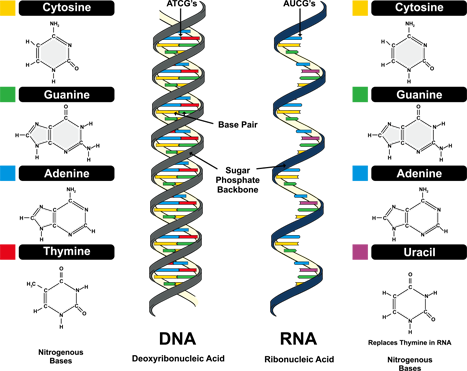
\includegraphics[width=6cm]{dna.png}
\end{figure}
\newpage
\begin{table}[h!]
\centering
% 列の定義を調整し,自動で改行されるようにしました
\begin{tabular}{|p{4cm}|l|p{2.5cm}|p{5cm}|}
\hline
\multicolumn{1}{|c|}{\textbf{名称}} & \multicolumn{1}{c|}{\textbf{糖}} & \multicolumn{1}{c|}{\textbf{塩基}} & \multicolumn{1}{c|}{\textbf{備考}} \\ \hline
\textbf{DNA} \newline (デオキシリボ核酸) & デオキシリボース & アデニン (A)チミン (T)  シトシン (C)グアニン (G) & 遺伝子の本体.2本のポリヌクレオチド鎖の塩基(AとT, GとC)の間で水素結合をつくり,二重らせん構造を形成. \\ 
\hline
\textbf{RNA} \newline (リボ核酸) & リボース &アデニン (A)ウラシル(U) シトシン (C)グアニン (G)  & DNAから遺伝情報を転写しタンパク質を合成する.(発現) \\ 
\hline
\end{tabular}
\caption{DNAとRNA}
\end{table}
\begin{figure}[H]
    \centering
    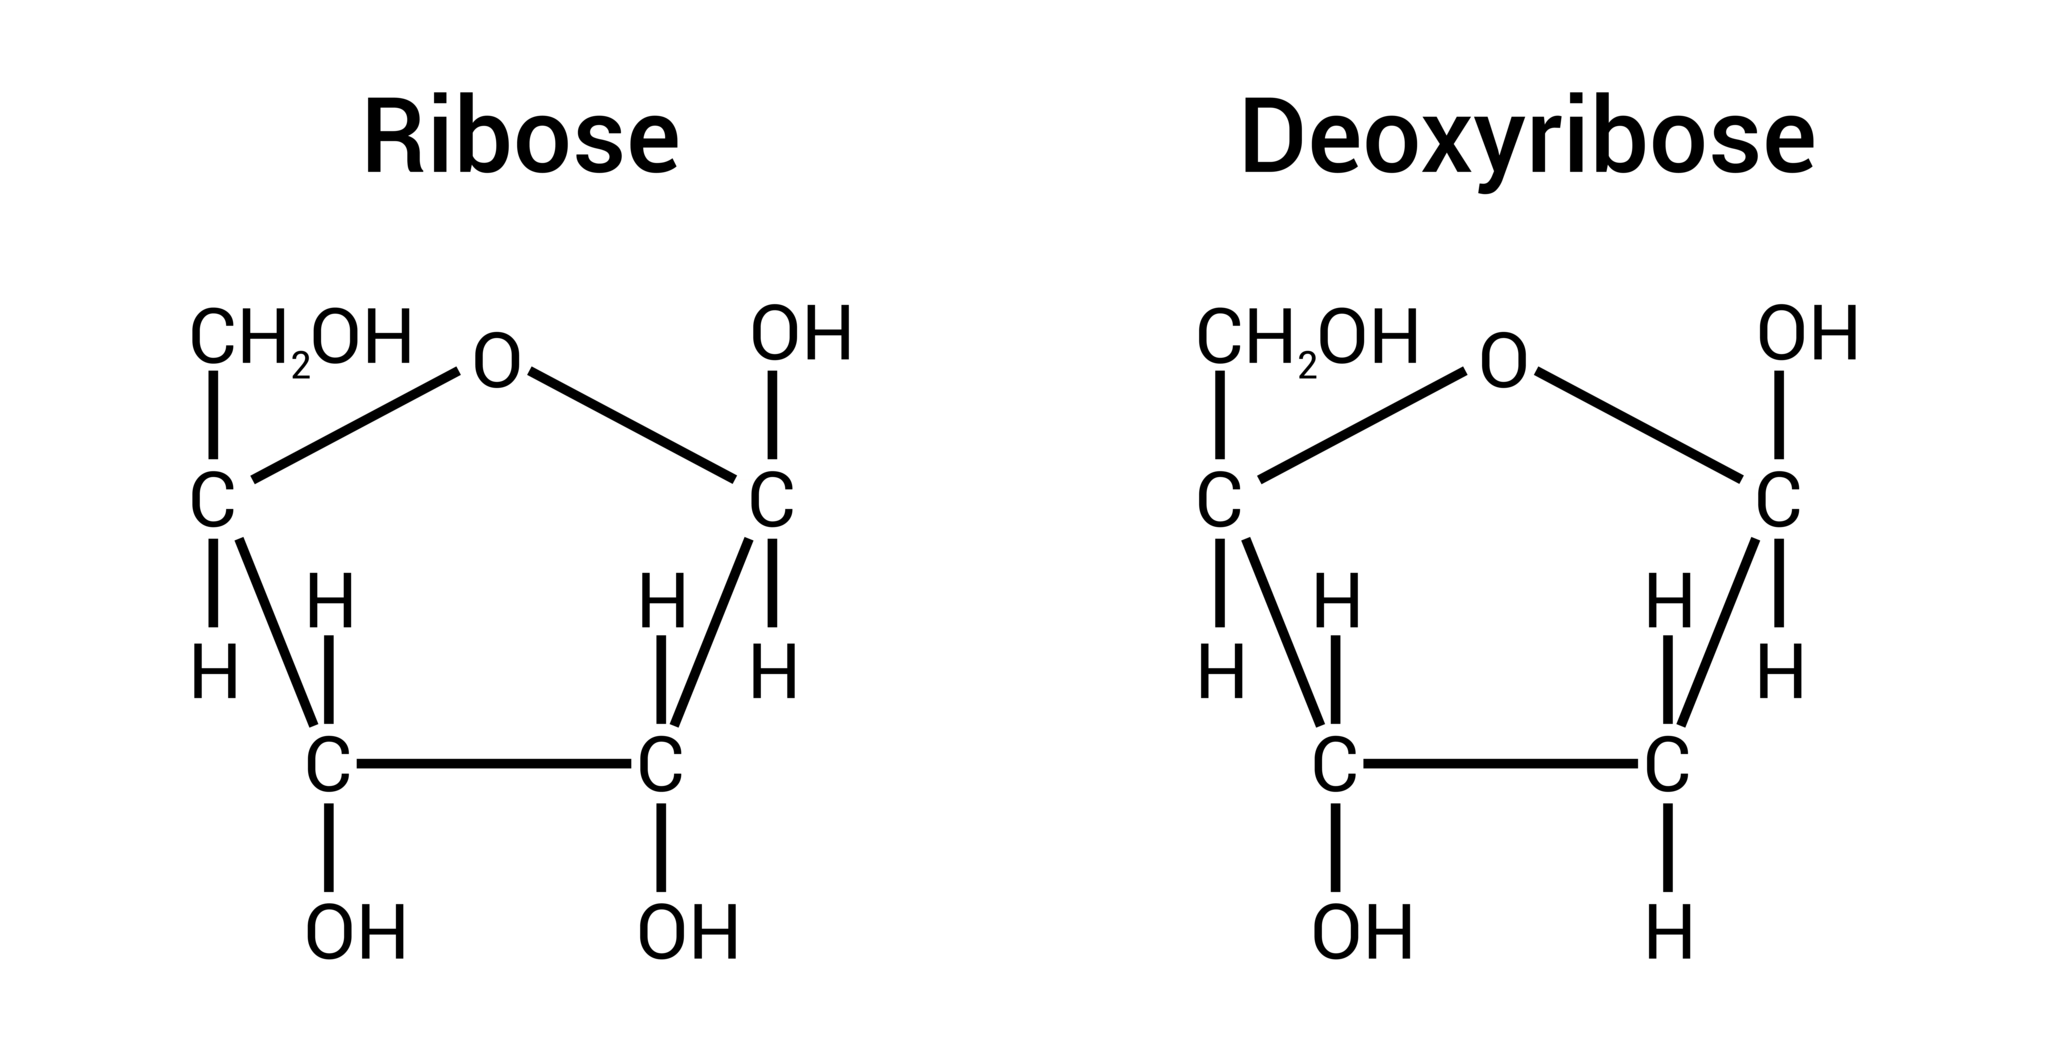
\includegraphics[width=10cm]{ribo-su.png}
\end{figure}
\ascboxA{\textbf{ ATP (アデノシン三リン酸)}}
\begin{itemize}
    \item[①] 塩基(アデニン)と糖(リボース)が結合したアデノシンにリン酸3分子が結合した物質.ヌクレオチドの一種である.
    \item[②] ATPが加水分解されるときに放出されるエネルギーが,生物のエネルギー源となる.
    \[ \text{ATP} + \text{H}_2\text{O} \longrightarrow \text{ADP (アデノシン二リン酸)} + \text{H}_3\text{PO}_4 \quad \Delta H < 0 \]
\end{itemize}



\end{document}